\section{What the recipe is not, and what the evidence supports}
\label{sec:recipe}

\subsection{The mirror-descent hypothesis does not survive the ternary loop}
\label{sec:rmd}

A natural reading of the residual---weights that moved but stayed quantized---is
that training used a large-$q$ mirror map or regularized mirror
descent~\citep{rmd,rmd2,proximalmf}: a potential $|w|^q$ with $q \gg 1$ pulls
weights toward magnitude attractors while distillation preserves the function,
so the final ternary projection becomes nearly lossless. The hypothesis is
attractive because it is testable with a single change to the optimizer.

We test it in the strongest configuration: inside the ternary loop, on the
1.7B canary, with the mirror-map update enabled at $q{=}16$ with a shell
parameter of $0.020$, against an otherwise identical straight-through control.
The deployed metric is the student-to-teacher perplexity ratio. The mirror-map
arm is worse at \emph{every} checkpoint (Table~\ref{tab:rmd}), and a retest in
the rotated basis also loses to the control ($8.54\times$). Earlier
encouraging mirror-map results were obtained in a different, projection-based
metric on full-precision masters, which is not the quantity that matters for a
deployed ternary model; in the deployed metric the hypothesis is falsified.

\begin{table}[t]
\caption{Mirror map inside the ternary loop (1.7B canary, deployed perplexity
ratio to teacher). The mirror-map arm is worse at every checkpoint.}
\label{tab:rmd}
\begin{center}
\begin{tabular}{lcccccc}
\toprule
step & $500$ & $1000$ & $1500$ & $2000$ & $2500$ & $3000$ \\
\midrule
STE control & $16.23$ & $14.62$ & $5.69$ & $4.94$ & $3.93$ & $\mathbf{2.93}$ \\
STE $+$ mirror map ($q{=}16$) & $94.53$ & $46.45$ & $44.34$ & $65.05$ & $55.66$ & $23.01$ \\
\bottomrule
\end{tabular}
\end{center}
\end{table}

\paragraph{Why it cannot be a tuning problem.}
The failure has a shape explanation. A mirror map forms a single magnitude
shell at $|w^{\star}| = \eta^{1/(q-1)}$, i.e.\ a unimodal prior on $|w|$.
Binary weights live on one shell: a single-well force at that magnitude is
exactly right, and the sign decides the side. Ternary needs mass at $0$ and at
$s$---a bimodal magnitude distribution---so a single-well force drains the zero
shelf no matter how it is tuned. Figure~\ref{fig:rmd-wells} shows the
mismatch; Figure~\ref{fig:rmd-shell} shows the distributions it acts on: after
rotation, the parameter that is optimized and ternarized is near-Gaussian, so a
coordinate-wise magnitude prior acts on a distribution that no longer carries
the original weight structure. Consistent with this, the released zero
fraction is what the absmean rule predicts from the weight distribution's shape
alone ($0.3276$ measured; $\sim 0.309$ near-Gaussian, $\sim 0.328$ at the
measured kurtosis), not the signature of a formed attractor
(\S\ref{sec:format}).

\begin{figure}[t]
\begin{center}
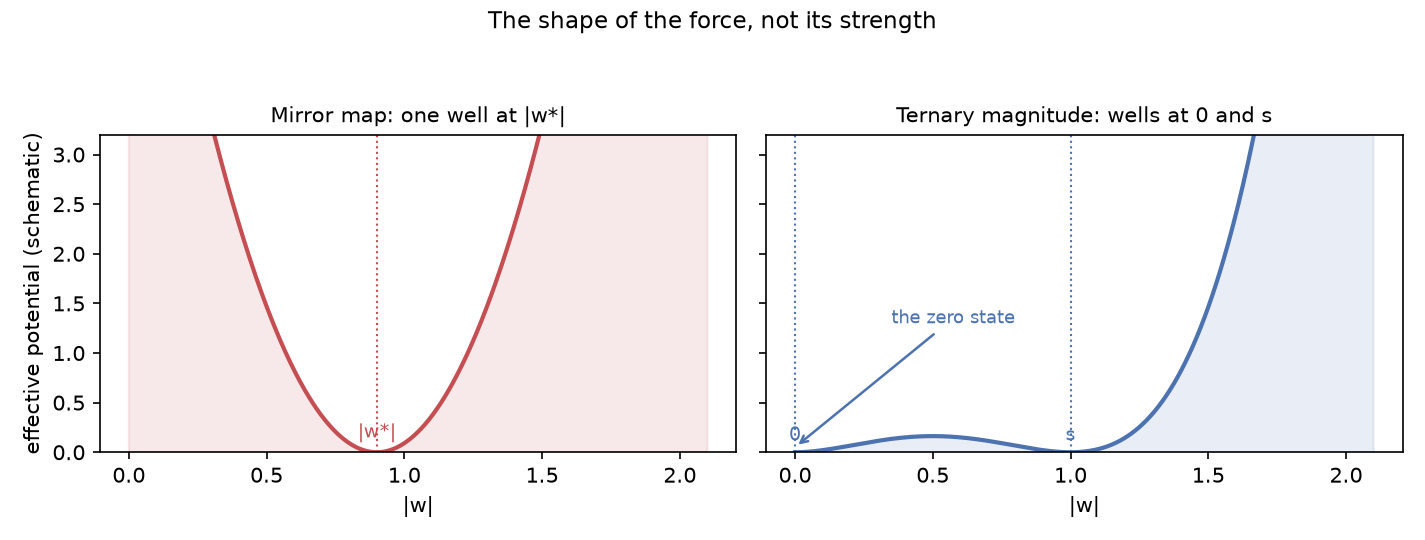
\includegraphics[width=0.85\linewidth]{figures/rmd-wells.png}
\end{center}
\caption{Schematic effective potential in magnitude. Left: the mirror map has
a single well at $|w^{\star}|$. Right: ternary needs two wells, at $0$ and
$s$; a single-well force cannot populate the zero basin.}
\label{fig:rmd-wells}
\end{figure}

\begin{figure}[t]
\begin{center}
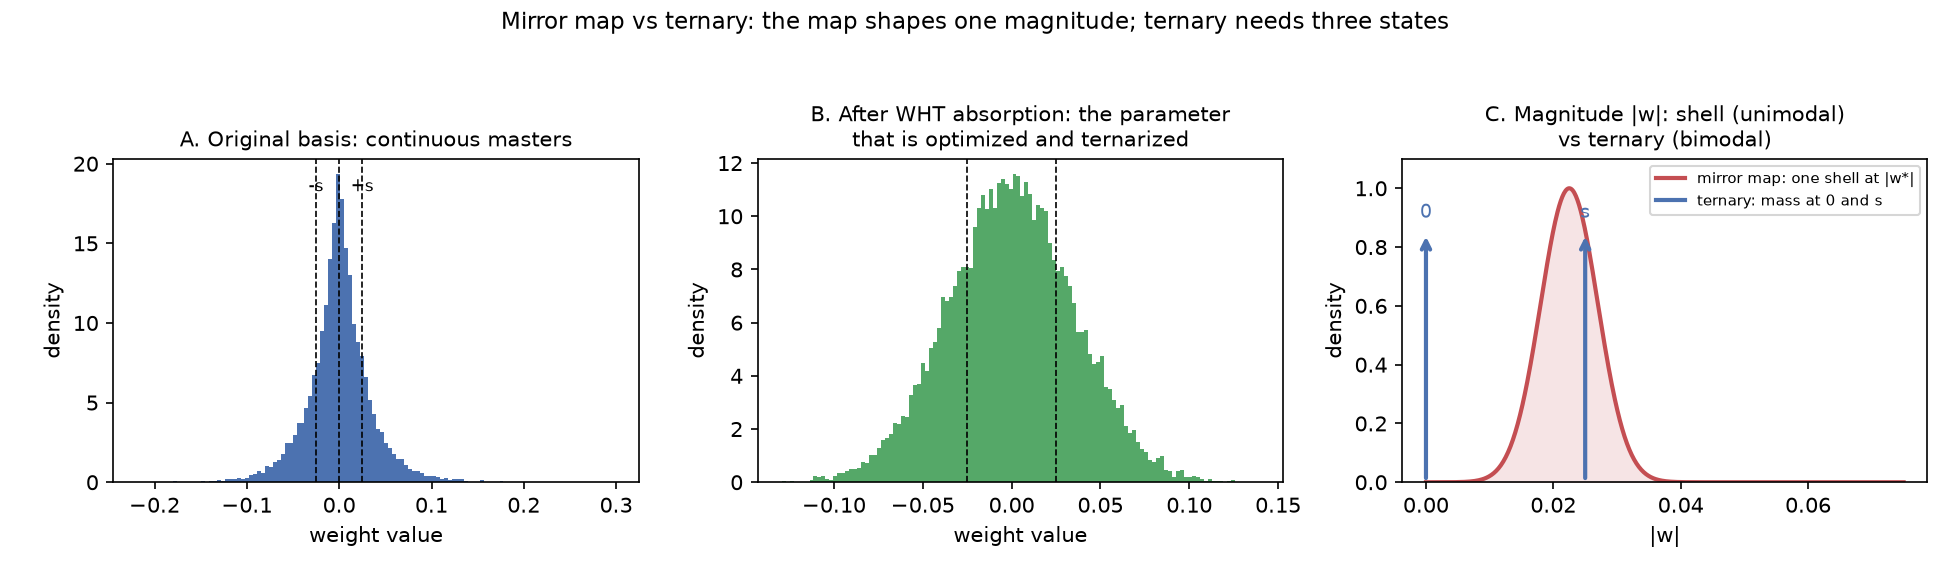
\includegraphics[width=\linewidth]{figures/rmd-shell-vs-ternary.png}
\end{center}
\caption{(A)~Continuous masters in the original basis with the ternary grid.
(B)~After the rotation is absorbed: the parameter that is optimized and
ternarized. (C)~The magnitude each method shapes; the mirror map forms one
shell, ternary needs mass at $0$ and $s$.}
\label{fig:rmd-shell}
\end{figure}

\paragraph{What the evidence supports.}
Putting the pieces together---the basis and format are public and exactly
recoverable; the residual is trained weight movement, not error compensation;
the zero band is the quantizer's band; the quality gap is total when the codes
are replaced; the mirror map fails in the loop---the best-supported account of
the release is the conventional one: \emph{rotation inside the training loop,
a ternary quantizer with a straight-through estimator, distillation from the
full-precision teacher, and a managed learning-rate schedule}. Mirror descent
belongs to the intellectual lineage of the mechanism, in particular the binary
case, but our experiments do not support it as the algorithm this model runs.

\subsection{The 1.7B pilot, and a holdout leak that retracts our own number}
\label{sec:pilot}

To price the remaining route we ran the conventional recipe on a
Qwen3-1.7B canary with the student and teacher on one card, distillation
temperature $2$, and a fixed evaluation set. The metric is the student-to-teacher
perplexity ratio (lower is better); retention is its reciprocal.

We have to open this subsection with a retraction. The first run of this pilot
reported $1.103\times$ ($90.6\%$ retention). A later audit found that the
harness sampled evaluation windows from the training pool---every evaluation
window had been seen roughly seventeen times during training---so the number
was a training-set measurement. A first correction ($1.219\times$, $82.0\%$)
turned out to be contaminated too: the holdout exclusion and the evaluation
call disagreed on sequence length, so the ``held-out'' evaluation still read
training data. Both numbers are retracted. On a clean multi-region holdout
(eight disjoint regions, $32$k tokens), the plain straight-through control sits
at $2.09\times$ mean ($\sim$48\% retention, range $1.55$--$2.71\times$). The
gap was larger than first reported, and the localization of
\S\ref{sec:mechanism} is what survives: the missing quality is training, not
quantization.

Under the clean holdout, the ablations behave as expected. Rotation inside the
loop is the single largest lever ($2.09\times \rightarrow 1.37\times$ at $5000$
steps); training longer improves it ($1.2152\times$, $82.3\%$, at $10{,}000$
steps); adding a managed decay schedule reaches $1.1052$--$1.1532\times$
($86.7$--$90.5\%$) depending on seed, though these are validation-selected
points. Corpus choice matters enormously: on WikiText~\citep{wikitext}, with an
in-distribution teacher, the same recipe at iso-convergence lands at
$1.5731\times$ ($63.6\%$) for 1.7B and $1.9263\times$ ($51.9\%$) for 0.6B,
rising with scale but far above the pre-registered bar. The 4B rung was dropped
by decision, so the scaling question is not resolved
(Figure~\ref{fig:retention}).

\begin{figure}[t]
\begin{center}
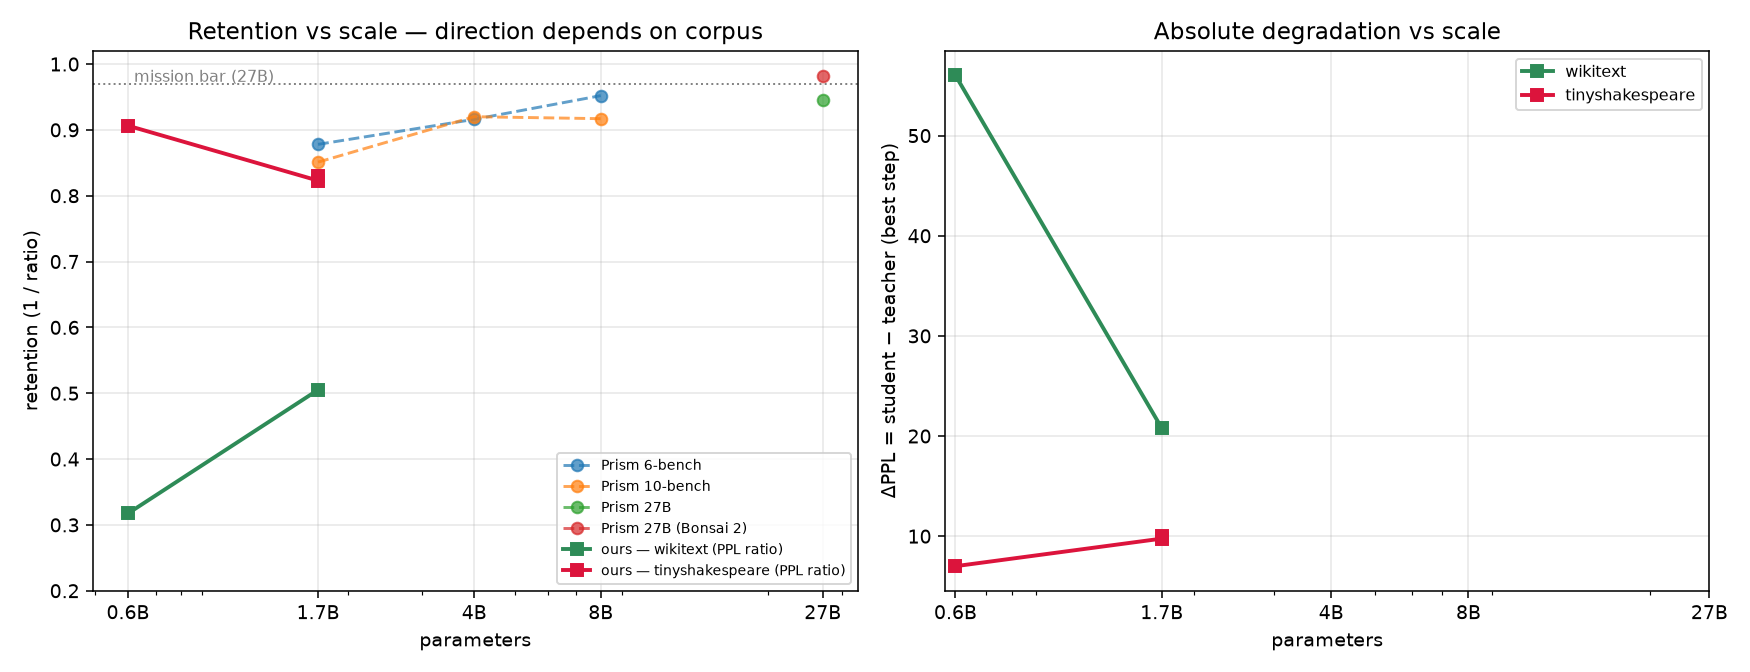
\includegraphics[width=\linewidth]{figures/retention-vs-scale.png}
\end{center}
\caption{Retention versus scale. Circles: the release's published benchmark
retention, which rises with scale. Squares: our canary's perplexity-ratio
retention on two corpora. The rulers differ (benchmark accuracy versus
perplexity ratio), so this is a same-scale sanity check, not a parity claim.}
\label{fig:retention}
\end{figure}

\paragraph{Where this leaves the gap.}
The residual that carries the quality is trained weight movement
(\S\ref{sec:mechanism}); every cheaper route has been eliminated; a local
per-layer distillation variant does not control global compounding; and the
canary, once its evaluation is clean, is further from the bar than first
stated. The remaining route to reproducing the released artifact is a full
end-to-end QAT/KD run at 27B, which we did not fund. What this study proves is
\emph{where} the gap is and what does \emph{not} close it---not that the recipe
reproduces the released numbers.
